\documentclass[11pt, letterpaper]{article}
\usepackage[utf8]{inputenc}
\usepackage{graphics}
\usepackage{graphicx}
\usepackage[francais]{babel}
\usepackage[T1]{fontenc} 
\usepackage[top=3cm, bottom=3cm, left=2cm, right=2cm]{geometry}
\usepackage{float}
\usepackage{url}
\usepackage{fancyhdr}
\usepackage[official]{eurosym}
\usepackage{comment}
\usepackage{hyperref}

\newcommand{\hmark}{\rule{\linewidth}{0.5mm}}

\begin{document}
\pagestyle{fancy}

\renewcommand{\headrulewidth}{1pt}
\rhead{}

\begin{titlepage}

\centering
\begin{figure}[t]
\begin{center}

\includegraphics[scale = 0.2]{upmc.png}
\end{center}
\end{figure}

\begin{center}
\par\vspace {2.5cm}
{\Huge\textbf{Rapport final : Hanabi\\*[0.25cm]}}   
\par\vspace {2cm}
{\Large\textbf{Université Pierre et Marie Curie\\ Projet ANDROIDE\\
               2015-2016}}                   
\par\vspace {2cm}
{\Large{Antunes Costa Gonçalves Daniel}}\\
{\Large{Assmann Catalina }}\\ 
{\Large{Hubert Cédric}}\\ 
{\Large{Wolfrom Matthieu}}\\
\end{center}

\end{titlepage}

\newpage

\tableofcontents

\newpage
\pagenumbering{arabic}

\section{Présentation du projet}

\subsection{Contexte}

\noindent 
Ce projet se déroule dans le contexte de l'UE Projet de première année de Master ANDROIDE de l'UPMC. Nous sommes un groupe de quatre étudiants qui doit mener à terme un projet proposé par leurs encadrants. Ce projet repose sur l'utilisation d'une intelligence artificielle qui exploite la logique épistèmique afin d'appliquer la meilleure stratégie possible pour le jeu Hanabi.

\subsection{Présentation du jeu Hanabi}

\noindent
Hanabi est un jeu de cartes coopératif composé d'un ensemble de cartes et de jetons. Les cartes représentent des feux d'artifice et les joueurs doivent collaborer afin de composer cinq feux d'artifice de couleur différente. On dispose au début de la partie de 8 jetons <<indice>> qui représentent le nombre d'indices auquel on a encore le droit, ainsi que 3 jetons <<éclair>> qui représentent le nombre d'erreur que l'on peut faire avant de perdre la partie. Les jetons sont retournés lorsqu'un indice est donné ou une erreur commise. Un jeton d'indice peut être remis sur son côté initial lorsqu'on défausse une carte.\\

\noindent
Personne ne connaît ses propres cartes, mais chacun voit les cartes des autres. En utilisant des indices et les cartes visibles, les joueurs doivent essayer de poser les feux d'artifice en suites croissantes de cartes de même couleur.\\

\noindent
Le score final est la somme des valeurs des dernières cartes posées pour chaque couleur.\\

\noindent
Pour réussir ce défi, chaque joueur peut à son tour soit donner un indice à un autre joueur, soit défausser une carte, soit jouer une carte.\\

\noindent
Un indice consiste à indiquer quelles cartes sont d'une certaine couleur ou d'une certaine valeur. Un indice négatif peut aussi être donné, indiquant qu'un joueur ne possède aucune carte d'une certaine couleur ou valeur. à chaque indice, un jeton <<indice>> est utilisé et donc retourné. Si le joueur choisit de défausser une carte, il regagne un jeton <<indice>>. Par contre, quand un joueur tente sa chance et joue une carte, il est possible que la carte ne complète pas la suite de sa couleur de feu d'artifice, dans ce cas un jeton <<éclair>> est retourné. Une fois que trois jetons éclairs sont retournés, le jeu est fini et les joueurs ont perdu.\\

\subsection{Objectifs}

\subsubsection{L'application}

\noindent
L'objectif de ce projet est de créer un logiciel qui permet à un joueur humain de jouer à Hanabi avec une ou plusieurs intelligences artificielles. \\

\noindent Le joueur pourra choisir le nombre de joueurs, entre deux et cinq. Pour une partie entre 2 ou 3 joueurs, chaque joueur a 5 cartes. Pour plus de joueurs, chaque joueur a 4 cartes. L'utilisateur peut choisir entre quatre intelligences pour chacun des joueurs virtuels.\\

\noindent L'interface graphique permettra à l'utilisateur de voir la partie, en visualisant les cartes de son équipe mais pas les siennes. Il pourra voir aussi la défausse et les indices donnés.\\

\noindent Il y aura des options pour sauvegarder la partie et la continuer ultérieurement. \\

\subsubsection{La logique épistémique}

\noindent Hanabi étant un jeu basé sur la coopération entre les joueurs pour permettre à chacun de connaître ses cartes et ainsi de les jouer. La logique épistémique est un moyen de représenter et de raisonner sur les connaissances d'un ou plusieurs agents, c'est donc l'approche qui a été retenue pour ce projet.\\

\noindent Pour faciliter la compréhension de notre  \hyperref[modelisation]{modélisation}, voici quelques bases sur la logique épistémique.\\

\noindent On considère la modalité $K_i$ pour chaque agent i. La notation $K_i(\varphi)$ signifie ainsi que l'agent i sait que la proposition $\varphi$ est vraie.\\

\noindent Les modèles de Kripke sont utilisés pour représenter les mondes possibles, où chaque proposition est donnée comme vraie ou fausse selon la relation définie. Le monde réel est l'un de ces mondes envisageables. Les mondes sont mis en relation pour chaque agent si ce dernier ne peut pas distinguer les mondes concernés à l'aide de ses connaissances.\\

On note alors :
\begin{itemize}
    \item Un univers $U$ contenant l'ensemble des mondes du modèle.
    \item Une relation d'accessibilité $\equiv_i$ pour chaque agent i.
    \item Une relation  $m \vdash \varphi$ qui indique que m vérifie la proposition $\varphi$. 
    \item Un modèle est ainsi noté $M=\{U, \{\equiv_1, ..., \equiv_m \} \}$\\
\end{itemize}
Une proposition $\varphi$ est valide dans un modèle $M$ si $\forall m \in U, m \vdash \varphi$, on le note alors $M \models \varphi$

\section {Expression des besoins - A REVOIR ?}

\subsection{Besoins fonctionnels}

\noindent
Le logiciel doit permettre à l'utilisateur de jouer une partie du jeu Hanabi avec d'autres joueurs artificiels. Pour ceci, nous avons besoin de créer les fonctionnalités suivantes : 

\subsubsection{L'interface Graphique}

\paragraph{Un menu d'accueil}

\begin{enumerate}

 \item  {Les règles du jeu}
 
  L'utilisateur peut cliquer sur ce bouton pour qu'on lui affiche les règles du jeu.\\


 \item  {Continuer une ancienne partie}
 
 L'utilisateur peut cliquer sur ce bouton pour qu'on lui affiche les parties sauvegardées et en choisir une pour la continuer.\\

 
 \item  {Commencer une nouvelle partie}

En cliquant sur ce bouton, le joueur voit une fenêtre où il doit préciser avec combien d'IAs il veut jouer (maximum 4 IAs). Il doit aussi préciser si les IAs jouent toutes avec la même stratégie ou avec des stratégies différentes.

\end{enumerate}

\paragraph{L'affichage de la partie}

\begin{enumerate}

\item  {Visualiser les cartes des autres joueurs}

 Les cartes des autres joueurs sont visibles par l'utilisateur.\\

\item  {Visualiser les jetons indices restants}

 Les jetons sont affichés sur la table et donc visible par l'utilisateur. Une fois utilisé, le jeton n'est plus visible.\\

\item  {Visualiser les jetons éclairs retournés}

 Les jetons éclairs sont tous affichés sur la table, retournés ou non.\\

\item  {Visualiser les cartes jouées}

 Les cartes jouées sont visibles sur la table.\\

\item  {Visualiser les cartes défaussées}

 Ce bouton permet à l'utilisateur de revoir les cartes défaussées. L'interface afficher toutes les couleurs des cartes défaussées et les numéros correspondants.\\

\item  {Visualiser les indices donnés pour les cartes de chaque joueur}

 A chaque indice reçu, l'utilisateur le voit affiché sur la carte concernée. Les indices sont soit une couleur, soit une valeur. L'utilisateur peut aussi voir les indices données aux autres joueurs, pour connaître leur base de connaissance de leur cartes.\\

\item  {Jouer une carte}

 L'utilisateur peut cliquer sur ce bouton et choisir la carte qu'il veut utiliser. La carte est donc affichée et est soit posée sur la table, soit défaussée si la carte ne convient pas. Si la carte est défaussée, un jeton d'éclair est retourné sur la table.\\

\item  {Défausser une carte}

 L'utilisateur peut cliquer sur ce bouton et après choisir la carte qu'il souhaite défausser. Elle est donc ajoutée à la pile de cartes défaussées, et un jeton d'indice est reaffiché pour pouvoir être réutilisé.\\

\item  {Donner un indice}

 Pour donner un indice, l'utilisateur clique sur ce bouton puis sur la main qui l'intéresse. Il choisi ensuite soit une couleur, soit une valeur, qui est attribuée aux cartes correspondantes. Il ne peut pas changer les informations déjà donnés par rapport à une carte. Un jeton d'indice est donc supprimé.\\

\item  {Sauvegarder la partie}

 L'utilisateur peut donner un nom à sa partie et la sauvegarder pour continuer à un autre moment.\\

\item  {Fin du jeu}

 La fin du jeu est affichée via une annonce. L'annonce affiche si l'utilisateur a gagné ou perdu. S'ils ont perdu, la raison est affiché (3 éclairs). S'il a gagné, son score est affiché. L'utilisateur peut ensuite choisir s'il veut faire une nouvelle partie, continuer une autre partie ou quitter le jeu.\\

\end{enumerate}


\begin{figure}[h]
\centering
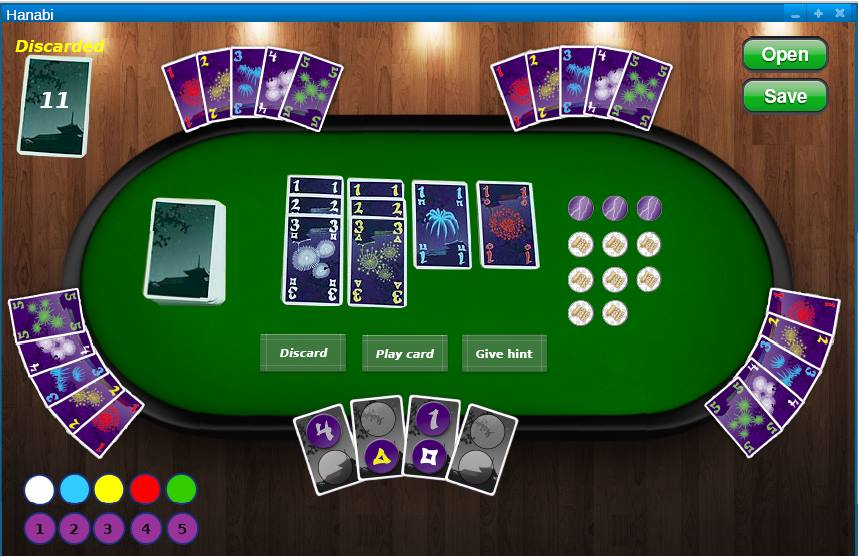
\includegraphics[scale = 0.4]{ihm.jpg}
\caption{Prototype d'interface graphique sur lequel on se base pour notre implémentation.}
\end{figure}

\subsection{Besoins non fonctionnels}

\noindent
L'intelligence artificielle doit décider de son prochain coup en un temps limité afin que la partie se déroule normalement. Il est donc indispensable que les IAs soient efficaces et optimisées. \\

\noindent
Nous avons réfléchi à plusieurs possibilités pour les IAs :\\

\begin{itemize}
    \item[$\bullet$] {\bfseries Une IA simple} : cette IA joue d'une manière basique: elle joue une carte valide si possible (quand elle connaît la carte, et elle peut être posée), sinon, elle donne des indices aléatoires tant que des jetons sont disponibles, dans le cas contraire elle défausse une carte (en priorité les cartes déjà posées ou les cartes sans indices).\\
    \item[$\bullet$] {\bfseries Une IA sans risque} : cette IA ne joue des cartes que quand elle les connaît. Dans le cas contraire, elle évaluera s'il vaut mieux défausser une carte ou de donner un indice et lequel.\\
    \item[$\bullet$] {\bfseries Une IA qui prend des risques} : cette IA est moins adverse au risque. En utilisant une heuristique, elle évalue les probabilité de réussite des différentes actions possible et choisi le meilleur coup. \\
    \item[$\bullet$] {\bfseries Une IA omnisciente} : cette IA connaît toutes les cartes (même les siennes), elle se concentre donc sur les priorités entre les différents coups possibles (jouer une carte qu'on connaît, défausser des cartes pour gagner des jetons <<indice>> ou donner des indices aux autres joueurs) 
\end{itemize}


\subsection{Critères d'acceptabilité du produit}

\noindent
Notre but est de simuler un jeu entre deux ou plusieurs joueurs, en utilisant des intelligences articifielles. Nous avons donc besoin d'avoir des IAs efficaces qui ne prennent pas trop de temps pour calculer leur prochain coup. Nos critères d'acceptabilité par rapport aux intelligences artificielles sont donc :\\

\begin{itemize}
    \item[$\bullet$] De permettre à l'utilisateur de jouer une partie de Hanabi sans devoir attendre trop longtemps pour son tour.\\

    \item[$\bullet$] L'intelligence artificielle est considérée comme efficace si elle atteint systématiquement un score entre 20 et 25 (le score maximum possible) en ne jouant qu'entre des IAs avec la même stratégie.\\
\end{itemize}

\noindent
Nous voulons aussi que le jeu soit facile et simple à jouer pour le joueur humain, donc une interface claire et compréhensible est indispensable. Il faut que toute personne soit capable de s'en servir. Nous voulons aussi avoir au moins une IA qui joue de façon réaliste plutôt que d'essayer de faire un score maximal.


\section{Conception}

\subsection{Déroulement du projet - EN COURS}

\noindent L'UE Projet se déroule pendant tout le semestre. Nous avons eu quatre mois pour l'analyser, le compléter et le tester. N'ayant jamais entendu parler de Hanabi, nous avons du nous en accointer (************************Is this sentence correct? ***************************). Pour commencer, nous avons acheté le jeu Hanabi sur Amazon. Cette livraison a pris quatre semaines, et nous a empêché de joueur et donc connaître le jeu au début du projet. 

\subsubsection{Organisation du projet}

\noindent En attendant l'arrivée du jeu, nous avons découpé les tâches en deux. Il fallait travailler sur l'architecture du code et aussi rédiger le cahier des charges. En séparant notre groupe en deux binômes, nous nous sommes mis au travail.\\

\noindent En écrivant le cahier des charges, nous avons mis au clair les fonctionnements nécessaires pour la conception du jeu et nous a permis de réfléchir aux intelligences artificielles possibles, comme précisé dans \textbf{\textit{Besoins non fonctionnels}}. Nous avons aussi choisi un design pour l'interface graphique.\\

\noindent Parler des premieres classes qu'on a fait?

\subsubsection{Entraînement du technique}

\noindent A l'arrivée du jeu, nous nous sommes mis à jouer. Jouer un jeu entre amis pendant des heures, dans les yeux des autres étudiants, semblait amusant, mais pour nous c'était de la recherche. Étant ceux qui allait programmer des intelligence artificielles capables de bien jouer, il fallait savoir bien jouer. \\

\noindent Dès le début, nous avons eu des idées des méthodes pour avoir un meilleur score. Certaines étaient bonnes, d'autre moins. Par exemple, comme la carte cinq de chaque couleur existe en un seul exemplaire, nous l'avons considérée comme essentielle. Cependant, si on jette toutes les deux d'une couleur, nous n'aurons jamais besoin du cinq alors il ne sert à rien de le garder. Nous avons découvert que la technique doit s'adapter à chaque partie, avec certains conseils à suivre. \\

\noindent Donner la priorité au joueur le plus proche pour des indices\\

\noindent 

\subsubsection{Programmation}

\noindent Console dummyIA

\noindent Il fallait coder le jeu pour pouvoir jouer en console. D'abord nous l'avons codé dans \textbf{\textit{Partie}} et \textbf{\textit{PartieTerminal}} pour que deux personnes puissent jouer ensemble en affichant les cartes comme une liste. Sur le console, sans une première intelligence artificielle, c'était impossible de jouer proprement à Hanabi du au fait de ne pas pouvoir cacher les cartes des joueurs.\\

\noindent En conséquence, il nous fallait une IA d'essai qui pourrait joueur contre le jouer humain. Nous avons donc programmé un IA tout simple qui s'appelle \textbf{\textit{DummyIA}}.\\

\noindent Interface Graphique\\

\noindent SemiDummyIA\\

\noindent Améliorations IA\\

\noindent Tests et améliorations graphiques\\


\subsection{Architecture - A FAIRE}

\noindent
L'architecture de notre code (MVC), etc.

\subsection{Diagrammes de classe - A FAIRE}


\section{Logique et stratégie}

\subsection{Rappels de logique}

\subsection{Choix de modélisation - A REFAIRE}\label{modelisation}

\noindent
Ici le but est d'identifier chaque situation de jeu possible par un monde de Kripke.\\

\noindent
La première étape est de modéliser les mondes liés à la main (combinaison de 4 ou 5 cartes sans ordre) du joueur, c'est à dire toutes les mains possibles en prenant en compte les cartes vues, déjà jouées ou déjà défaussés. L'agent correspondant au joueur hésite donc entre tous ces mondes possibles.\\

\noindent
Notre structure de Kripke est donc:\\

$\mu=\{U,\{R_{1}\},I \}  $\\
$   U=\{M_{1},...M_{m} \}   $\\

\noindent
$R$: A ce stade, $R_{1}$ connecte tous les mondes, on suppose que l'on ne génère pas les mondes qu'il sait déjà impossibles.\\

\noindent
$I$: On note    $C_{j,c,v}$ la variable affirmant que le joueur j possède une carte de couleur c et de valeur v. Pour n joueurs, un monde $M_{i}$ contiendra donc toujours un nombre de variables $nv=n*4 | n>3$ ou $nv=n*5 | n<4$\\

\noindent
A ce niveau de modélisation, on peut déjà envisager des prises de décisions probabilistes simplement en comptant le nombre de mondes dans lesquels faire telle action aurait un impact positif.\\

\noindent
Ensuite, il est également possible pour le joueur de modéliser les mondes entre lesquels il pense qu'un autre joueur hésite. Appelons le joueur qui réfléchit $j_1$ et celui sur lequel il porte sa réflexion $j2$. Cela pose problème car ce $j_2$ dispose d'informations que n'a pas $j_1$ (ses propres cartes), mais on peut tout de même savoir que des mondes sont impossibles grâce à l'information commune aux 2 joueurs (les cartes des autres joueurs, les cartes jouées, les cartes défaussées, les indices donnés).
Pour cela, on peut se baser sur les formules de la logique propositionnelle, auxquelles on ajoute la modalité de la connaissance: $K_j$ Les atomes sont représentés sous la forme :$\Phi_{j,c,c_1,v_1}$ tels que "la carte $c$ du joueur $j$ a la couleur $c_1$ et la valeur $v_1$". L'utilisation de l'axiome de connaissance est donc   $K_j(F)$ est vrai dans un monde $M$ si tous les $M'$ successeurs de $M$ pour la relation $R_j$ satisfont $F$. Ce raisonnement peut être appliqué pour chaque autre joueur.\\

\noindent
On a donc maintenant:\\

$\mu'=\{U',\{R_{1},...,R_{n}\},I' \} $\\

$U'=\{M_{1},...M_{m'} \} $\\

\noindent
Pour les relations $R_{i}$, il faut se dire que le joueur $i$ n'hésite qu'entre les mondes où toutes les cartes sont identiques sauf les siennes.\\

$   \forall i \in [2,...,n] ,  \forall (M_{j},M_{k}) \in U'*U',$\\

$R_{i}(M_{j},M_{k}) 
\equiv
\forall l \in [1,...,n]|l \ne i,  \forall C_{l,c_1,v_1} \in  I(M_{j}), \forall C_{l,c_2,v_2} \in  I(M_{k}), c_1=v_1, c_2=v_2    $\\

\noindent
Ensuite, il faut tenir compte des indices donnés par les joueurs qui sont des "annonces publiques" qui viennent enrichir la connaissance commune à tous les joueurs. Grâce à ces annonces et aux formules proposées plus haut, il est possible de supprimer des membres des relations (graphiquement, cela correspond à supprimer des arrêtes du graphe), et donc certains monde deviennent impossibles.

\noindent Modélisation carte par carte\\

\noindent
Cette fois, l'objectif est de créer des structures de Kripke pour chaque carte plutôt que pour chaque situation. Ainsi, sans information, il y aurait 25 mondes pour chaque carte. On peut ensuite tenter d'appliquer les mêmes raisonnements que dans la modélisation exhaustive.\\

Univers de la i-ème carte du joueur $j$:\\

$   \mu_{i,j}=\{U,\{R_{1},...,R_{n}\},I \}  $\\

$   U=\{M_{1},...M_{m} \}   $\\

$I$: chaque monde contient 2 variables, une pour la couleur et une pour la valeur. \\

$\forall M \in U, I(M)=(c,v)|c\in[rouge,bleu,vert,jaune,blanc],v\in[1,...,5]$\\

\noindent
Cette approche peut être utilisée comme la précédente pour choisir les coups à jouer de manière probabiliste. Cependant, si l'on veut essayer de raisonner sur la connaissance des joueurs, il est nécessaire de mettre en relation tous ces univers, et on en revient donc à la complexité de la modélisation exhaustive.

\subsection{Stratégies envisagées}

\subsubsection{Situations de jeu interessants - A FAIRE}

\subsubsection{Intelligences artificielles - A FAIRE}

\noindent \textbf{Fonctionnement du DummyIA}\\

\noindent Cette IA est la plus simple des IAs. Elle n'est pas très efficace mais elle a servi comme une base sur laquelle baser la prochaine IA.\\

\noindent DummyIA ne joue une carte que si elle connaît la carte et la carte est jouable. Si elle n'a pas de carte jouable et il reste des jetons indices, elle donnera un indice aléatoire à un joueur aléatoire. \\

\noindent Sinon, elle va défausser une carte. Les cartes inutiles, c'est-à-dire une carte connue où la même a déjà été posée sera prioritaire pour la défausse. Hormis ce cas, elle va jeter les cartes sans indices, et en dernier recours, aléatoirement.\\

\noindent \textbf{Évaluation du DummyIA}\\

\noindent Cette IA n'est pas efficace. 


\noindent \textbf{Fonctionnement de SemiDummyIA - A FAIRE Cédric}\\

\noindent
L'objectif de cette IA était de reprendre les principes de DummyJoueurIA en améliorant les indices donnés. Cependant, nous avons au fur et à mesure de sa conception incorporé des idées supplémentaires(décrites dans les paragrahes suivant), ce qui a aboutit à une IA\\

\noindent
Cette IA suit un algorithme précis.\\

\noindent Au début de son tour, si elle a une carte jouable immédiatement, elle la joue.\\

\noindent Si ce n'est pas le cas et qu'il reste des jetons d'indice, elle essaie d'en utiliser un. Pour cela, elle parcourt les mains des autres joueurs à la recherche d'une carte jouable. Si elle en trouve une, et que le joueur possédant la carte ne connait pas sa valeur, l'IA donne cet indice. Si elle connait la valeur de la carte, mais pas sa couleur, alors l'IA donne l'indice sur la couleur. Après le parcours des mains, si aucun indice n'a été donné (parce qu'aucune carte n'était jouable ou parce que celles jouables étaient déjà complétement connues par leurs propriétaires), alors l'IA donne un indice aléatoire.\\

\noindent Dans le cas ou il ne reste plus de jeton d'indice, l'IA va chercher à défausser une carte. Dans ce but, elle regarde dans un premier temps si, parmi ses cartes, elle sait que l'une d'entre elle est "défaussable"(c'est à dire qu'une carte identique a déjà été jouée ou qu'elle ne sera jamais jouable à cause des cartes défaussées jusqu'à maintenant).\\

\noindent Si elle en trouve une, alors elle choisit celle-ci. Dans le cas où l'IA ne trouve pas de carte défaussable, elle va essayer de défausser une carte sur laquelle on ne lui a pas donné d'indices. Il peut arriver qu'aucune carte ne lui soit complétement inconnue, la carte à défausser sera alors choisie aléatoirement.\\

\noindent \textbf{Evaluation de SemiDummyIA - A FAIRE Cédric}\\
\noindent Nous avons simuler 200000 parties à 2,3,4 et 5 joueurs entre des SemiDummyIA, sans utiliser les cartes multicolores. Voici les résultats obtenus:\\

2 joueurs: Score max : 21 Score min : 1 Score moyen : 10.622325\\
3 joueurs: Score max : 20 Score min : 6 Score moyen : 14.24381\\
4 joueurs: Score max : 19 Score min : 7 Score moyen : 13.88206\\
5 joueurs: Score max : 18 Score min : 7 Score moyen : 13.363\\




\begin{figure}[H]
\begin{center}
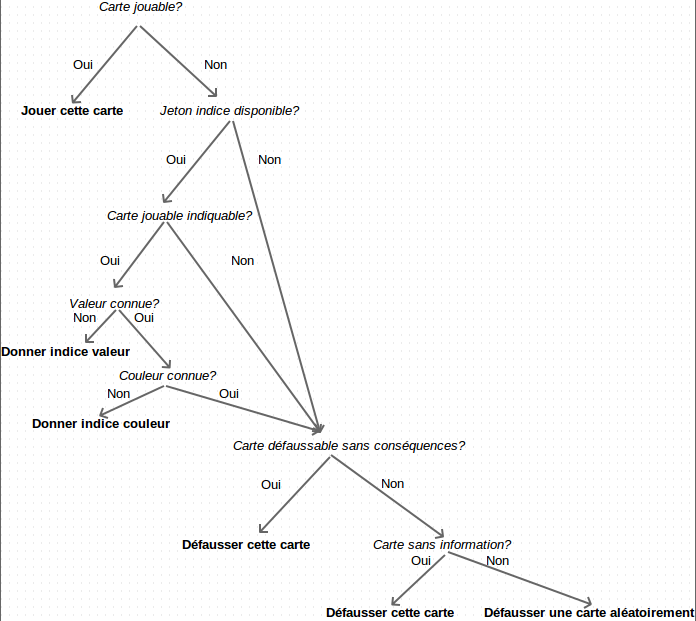
\includegraphics[scale = 0.3]{flow_chart_semidummy.png}
\end{center}
\end{figure}

\noindent \textbf{Heuristique IA - A FAIRE Cédric}\\

\section{Manuel d'utilisation}

\subsection{Lancer une partie}
\noindent En lançant le jeu, une fenêtre qui s'appelle \textbf{\textit{Bienvenue au jeu Hanabi}} s'ouvre. Dedans s'affiche deux boutons :\\

\begin{itemize}
    \item[$\bullet$] \textbf{\textit{Charger Partie}} - L'utilisateur peut choisir une partie existant sur son disque pour la continuer\\
    \item[$\bullet$] \textbf{\textit{Nouvelle Partie}} - Lance une fenêtre \textbf{\textit{Paramètres de jeu}}\\
\end{itemize}

\noindent \textbf{\textit{Paramètres de jeu}} propose à l'utilisateur de sélectionner le nombre de joueurs, choisir son pseudonyme et choisir le type d'intelligence artificielle pour chaque joueur. Il peut aussi cocher la case "Jouer avec les cartes multicolor". Ensuite il peut cliquer sur \textbf{\textit{Lancer la partie}} pour commencer. 

\begin{figure}[H]
\begin{center}
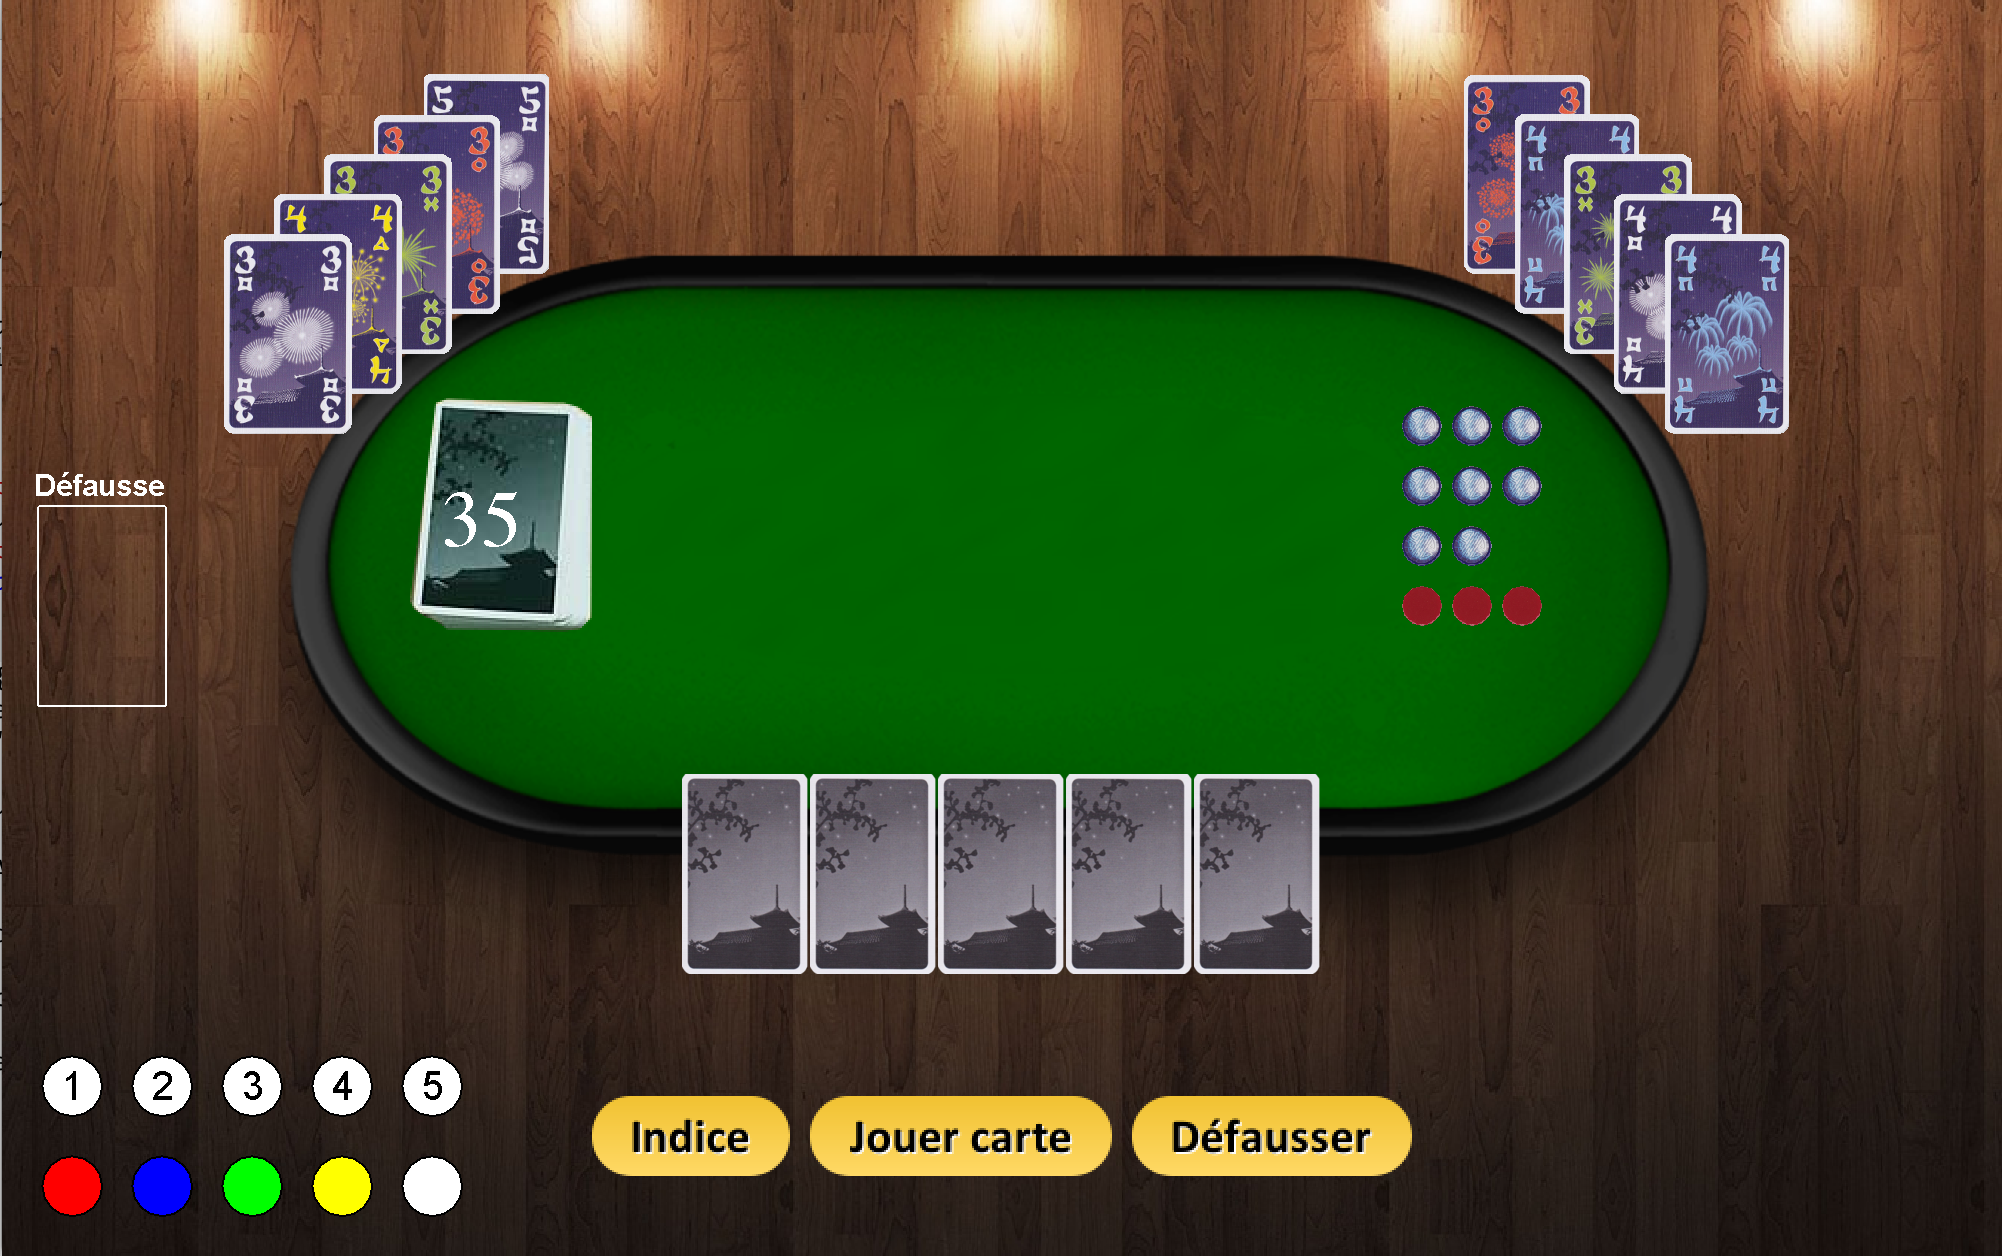
\includegraphics[scale = 0.5]{partie.png}
\caption{La partie lancée ressemblera à celle-ci}
\end{center}
\end{figure}

\subsection{Joueur une partie}

\noindent Une fois dans la fenêtre de la partie, le joueur verra trois boutons :\\

\begin{itemize}
    \item[$\bullet$] \textbf{\textit{Indice}} - Ce bouton permet au joueur de choisir un joueur à lequel il veut donner un indice. Son choix sera affiché par une bordure autour des cartes du joueur choisi. Ensuite il doit choisir soit une couleur, soit un nombre comme indice.\\
    \item[$\bullet$] \textbf{\textit{Jouer Carte}} - Ce bouton permet au joueur de choisir une carte qu'il souhaite jouer. Si son coup est réussi, la carte s'affiche sur la table. Sinon, un jeton éclair se retourne.\\
    \item[$\bullet$] \textbf{\textit{Défausser}} - Ce bouton permet au joueur de choisir une carte qu'il souhaite défausser. Cette carte s'affichera dans la pile de défausse.\\
\end{itemize}

\noindent Le joueur aura aussi l'option de cliquer sur la pile de défausse pour que les cartes défaussée s'affichent. Une fois qu'il veut revenir à la partie, il suffit de cliquer en dehors de la défausse.

\begin{figure}[H]
\begin{center}
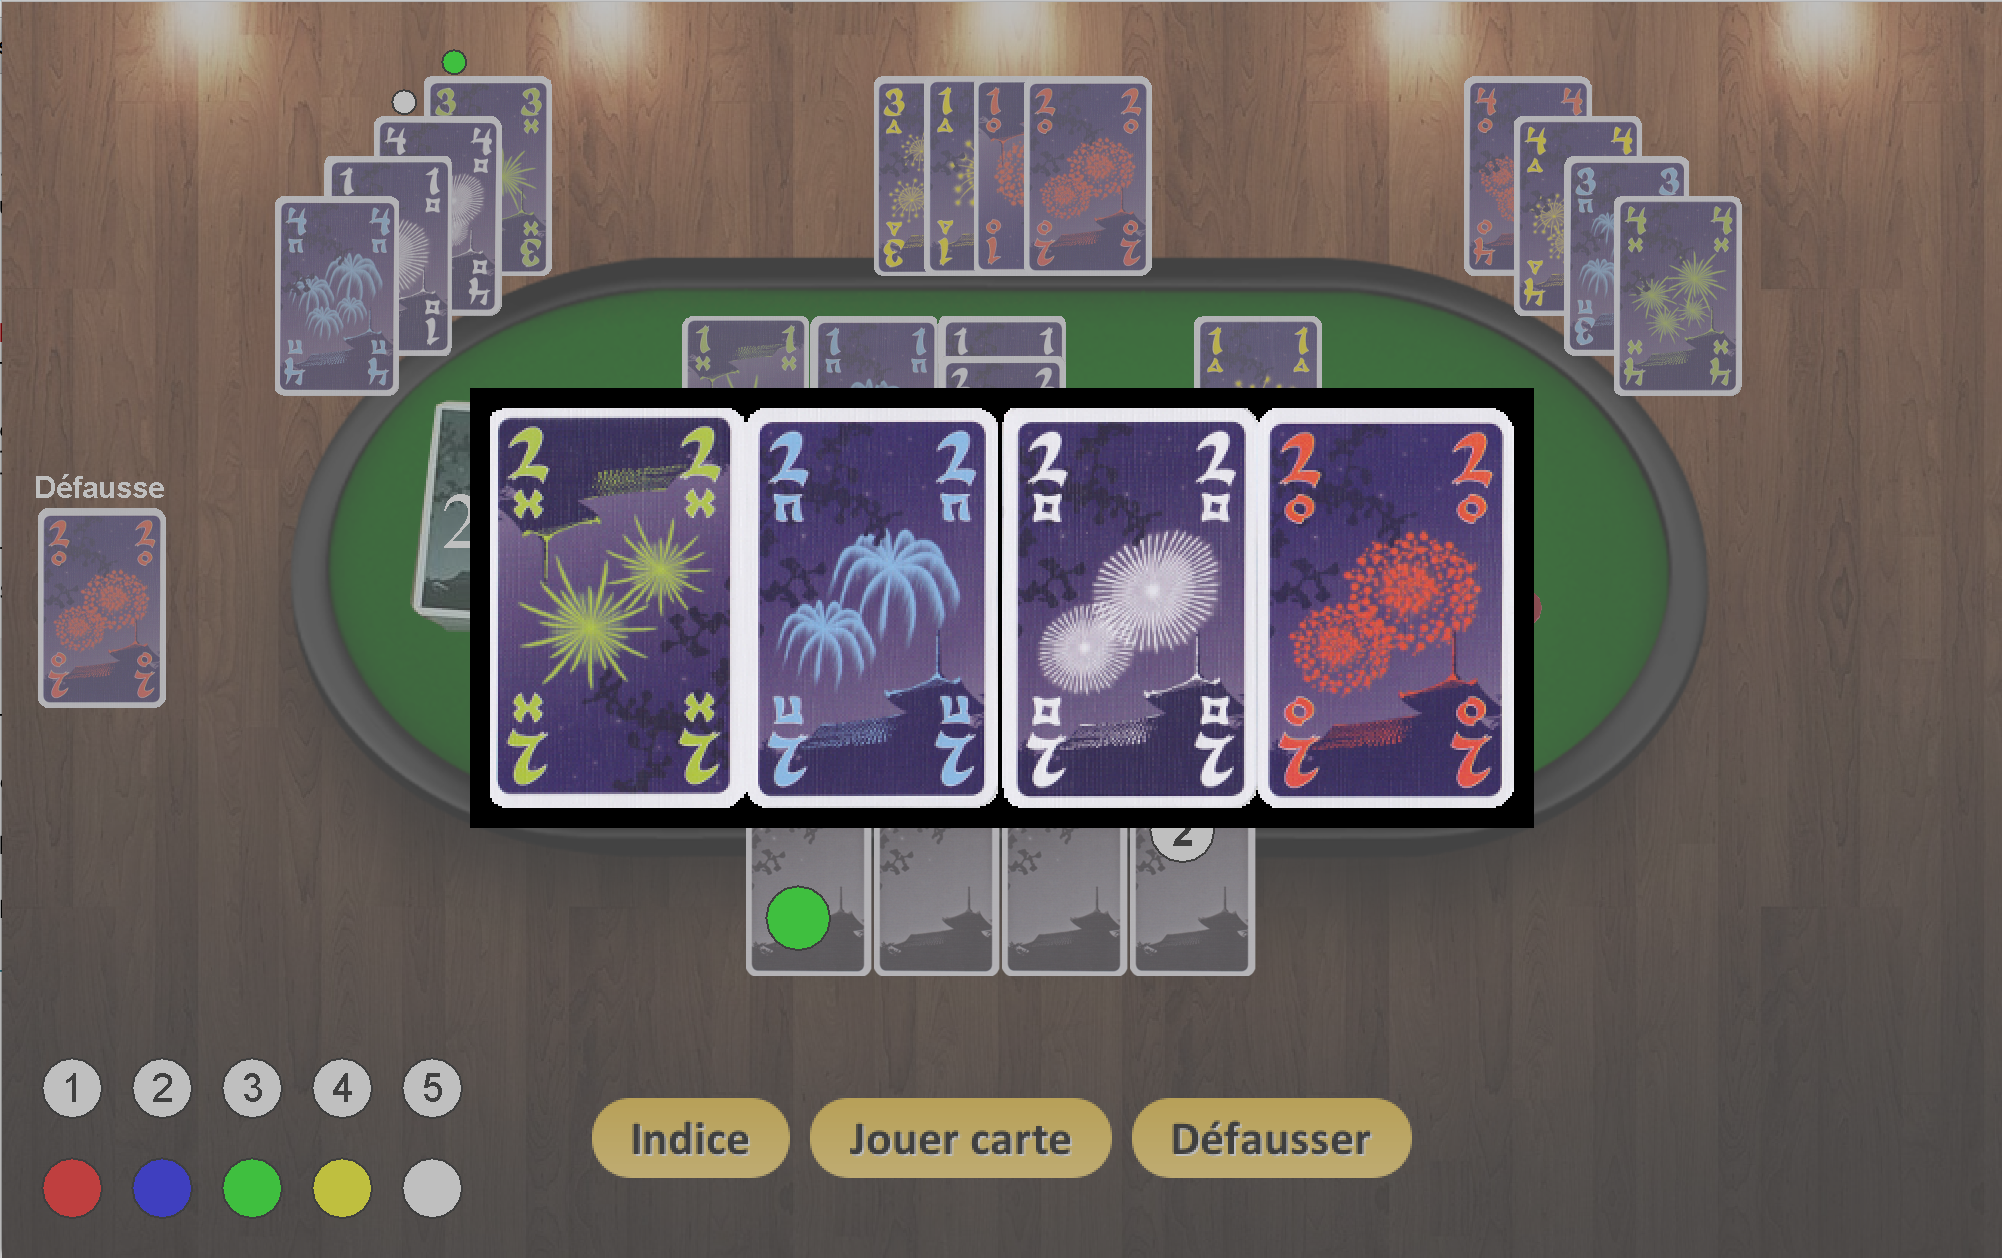
\includegraphics[scale = 0.5]{defausse.png}
\caption{La défausse d'une partie}
\end{center}
\end{figure}

\subsection{Sauvegarder une partie}

\noindent Pour sauvegarder une partie, l'utilisateur a deux choix. Soit il peut faire "Ctrl + s", soit il peut aller dans "Fichier" et cliquer sur \textbf{\textit{Enregistrer Partie}}.

\subsection{Fin de la partie}

\noindent A la fin de la partie, une fenêtre s'ouvrira pour déclarer si le joueur à gagné ou perdu. Dans les deux cas, il aura le choix entre trois boutons : \textbf{\textit{Nouvelle Partie}}, \textbf{\textit{Charger Partie}} et \textbf{\textit{Quitter}}.\\

\noindent Si le joueur à gagné, la fenêtre affichera aussi son score final.

\section{Tests - A FAIRE}

\section{Conclusion - A FAIRE}

\subsection{Difficultés rencontrées}

\subsection{Perspectives d'amélioration}

\end{document}
